\chapter[Exploring Needs in Persuasive Feedback] {Exploring Needs in\\ Persuasive Feedback}\label{chap:feedback_modalities}
% previous titles: 
% 	co-designing persuasive feedback 
% 	User-Centered Persuasive \\ Feedback
%TODO still not quite happy with the title, needs to be exactly what we did. 

% lingo: Narrative; ramification.

% FOCUS: Involve users in finding ways to provide better/more helpful/more actionable feedback. 
% learn from what they say explicitly, but also implicitly. 
% underlying persuasive principle: 
% \textit{social interaction} (team spirit) between the system and the users. (Forget et al).
% weirich and sasse / Sasse and Felchais --> Socio-Technical System. 
% participatory design methods, open questions, learning from feature requests.
% opportunity: past studies focused on retrospection. We involve users in creating new solutions without a basic starting point. 

% theoretically, magdalena's BA topic could be worth mentioning, too. 
% GOALs.
% 	Design nudges without letting users become aware of that. 
% 	Evaluate 

The overall goal of this thesis is to support users in how they interact with passwords. As a sub-goal, we wanted to help those users who want to handle password management on their own, i.e. without a password manager. We set out to achieve this goal by studying the design space of password feedback mechanisms like password meters. There have been many design proposals already and numerous evaluations. However, the design-space appears rather narrow if we only look at existing solutions, and many have not achieved the envisioned level of support. Therefore, we posit that the design-space needs to be opened up and show more width. To get there, looking at the requirements of password feedback is a necessary first step. Previous solutions have seldom reported a structured requirement elicitation based on user research. Thus, before designing and implementing support strategies outside of the usual spectrum we aimed to first understand the needs and expectations that users may have about password feedback. We tried to learn from their feature requests and their own proposals to be able to inform future design decisions. In particular, we posed the following broad research questions:

\begin{itemize}
	\item[RQ1] What do users \textit{expect} from password support tools during account creation (explicit) and what do they really \textit{need} (implicit)?
	\item[RQ2] How can we design password feedback in novel ways outside of the visual password meter and verbal real-time feedback spectrum? % Which alternative feedback solutions might be feasible to influence password selection? What individual roles do verbal and non-verbal feedback play?
	\item[RQ3] How can we leverage the interplay between feed-\textit{forward} and feedback?
\end{itemize}

%Goals: Help users create passwords that they can handle without a PWM (see previous chapter \ref{chap:mm_pwm}),
%RQs: how can we leverage persuasive design strategies for that? Are PW meters the right (and only) way?
%Method: \textbf{Design research about requirements and ``other ways'' to help users through improved feedback}.
%Practical Issues: see section on running password studies
%Ethical issues: collect plain text passwords? tried in bandwagon study, but there's some resentment. 


%Storyline:
%
%%(Intro: 1-2 pages)
%Problems:
%- nudging approaches have become stale
%- some solutions don't focus on the core goals like stronger passwords and/or less reuse
%- we found no formal requirement elicitation in the literature.
%
%Goals:
%- what do users say they need? derive solutions and design lenses from that. 
%- explore solutions that go beyond password meters. (THATS AN OVERALL GOAL)
%- put the users first and early (very user-centric)
%- learn from their design solutions (co-design) to inform future design decisions.
%
%
%what this chapter can realistically achieve: 
%verbal feedback: what is required. qualitative stuff (hint at suggestion trustworthiness, personalization)
%nudging: both verbally and visually; dimension: cognitive bias (bandwagon)


%lightweight and rapid iterations

This chapter reports on a requirements- and design-exploration for password feedback, where we aimed to involve users early in the design process. The project was a collaboration between myself and Caroline Olsienkiewicz, respectively Katharina Schwarz. 

\section{Background and Context}

% very briefly.
Design dimensions / aspects of persuasive authentication: PAF Forget \etal \cite{Forget2007PersuasionEducationSecurity}, see mindmap

\begin{figure}
	\centering
	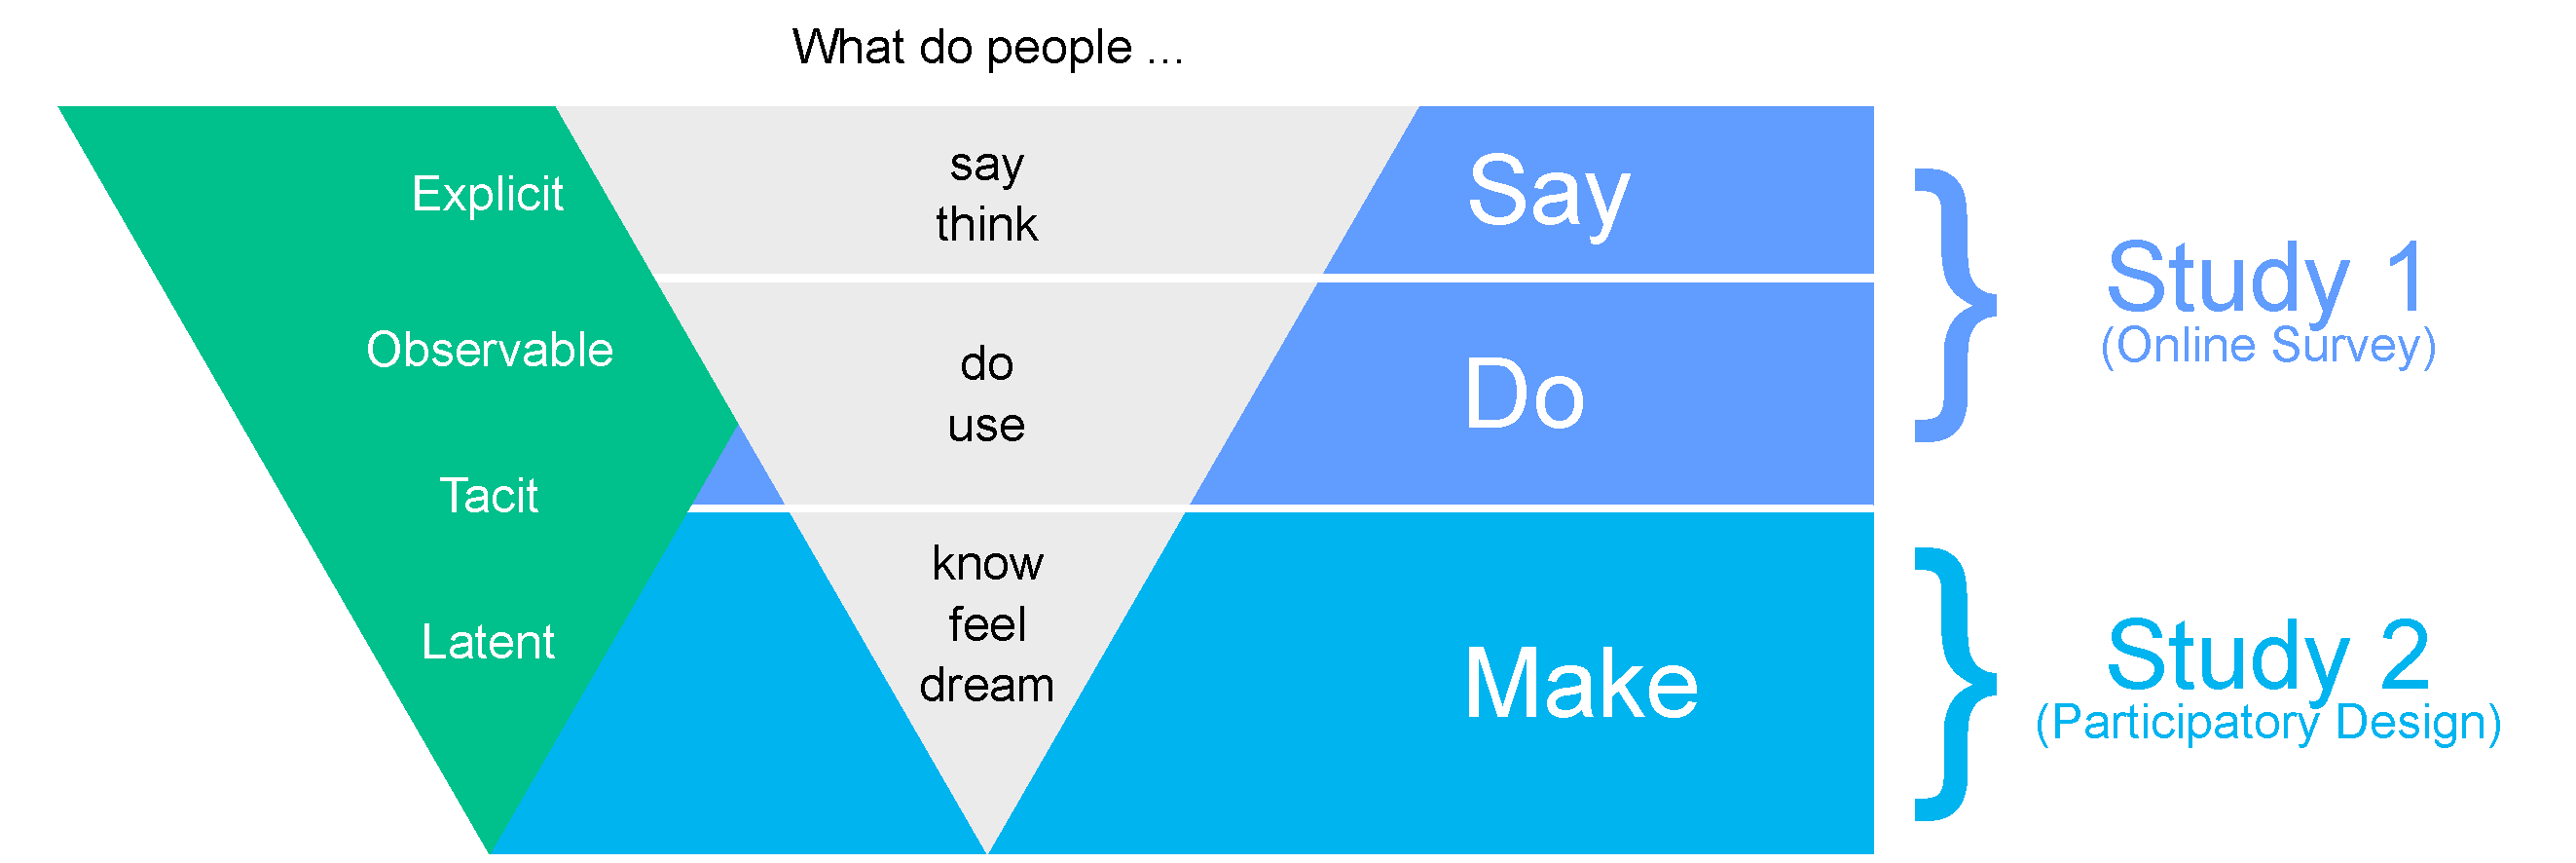
\includegraphics[width=\linewidth]{figures/co-design/exploration-overview}
	\caption{\label{fig:co-design:exploration-overview} Characteristics of user needs and how they show (adapted from  \cite{Sanders2002ParticipatoryDesign}). We explored explicit and observable needs with an online survey, and used a participatory design approach to learn from what users \textit{make}.}
\end{figure}


%%%%%%%%%%%%%%%%%%%%%%%
% CO DESIGN PART 1
%%%%%%%%%%%%%%%%%%%%%%%
\section{Explicit and Observable Needs}\label{sec:codesign:part1}
After the literature review (see Part \ref{part:related_work}), there were still open questions about user \textbf{expectations} regarding password strength feedback. Most studies went ahead to test new solutions quantitatively and rarely focused on the intrinsic needs to derive requirements for feedback. In other words, users were often involved late in the design process, although an earlier involvement could have led to different design decisions. Our goal in the first step of the co-designing process was gathering early insights to learn about the requirements of persuasive interventions in the realm of password authentication. 
%
To narrow down the focus of the requirements, it was important to consider a realistic use-case where the burden of password authentication is relatively high. From related work, we know that password changes are more frequent in work environments, because expiration-policies are still common there \cite{Inglesant2010TrueCostOfUnusablePolicies}. Frequent password changes lead to weaker practices, which might be mitigated by effective password feedback. To find out how we might improve such feedback, we used a lightweight, rapid survey with a large portion of open questions. In the following, we briefly describe the method and findings. 
%Goal: find out what users would expect from password feedback and what they would suggest doing to improve password selection for other users. 

%- Approach: Give users example of \textbf{verbal feedback} 
\subsection{Method}
We opted for an online survey to inform our requirement elicitation for the above described reasons and straightforward data collection. Our questionnaire was centered around the following core research questions:
\begin{itemize}
	\item What do users \textbf{expect} from password feedback?
	\item What do they \textbf{miss} in current solutions / interventions?
	\item How would they \textbf{improve} existing feedback?
\end{itemize}

%- qualitative survey 
%	- what works (subjectively) and what doesn't? It's not like people don't know that a study is about password feedback. strength isn't the only dimension. qualitative rating / assessment / perceived helpfulness.
%- What do they miss? 
%- What feedback ideas do they come up with?
%- motivate focus on work environment.
%- usually no choice,
%- expiration policies
%- many password changes leads to creativity deprivation (we should get rid of expiration anyhow)
%- pick up the specific questions b/c they were good

\subsubsection{Prototype}
To ensure that participants have a shared understanding of password feedback mechanisms, we created a small website featuring only a password field and textual feedback beneath. The underlying strength estimation and feedback phrases were based on the zxcvbn library. Warnings and suggestions that come with zxcvbn were translated to German and shown as the users typed inside the password field. The 26 warnings included statements like ``Names and surnames by themselves are easy to guess'' or ``Avoid repeated words and characters''. We tried to simplify the page as much as possible to minimize priming effects, although this was hard to achieve. In particular, we did not show any form of visual feedback to explore whether this is a need that participants mentioned often. Instead, we showed a password score in the form ``strength: 2/5''.  The page introduced the scenario (old password at work has expired) and asked participants to create a new password that would fulfill the composition policy of the participant's current employer. The composition policy, however, was not enforced, but we probed it in the questionnaire. We did not log the passwords whatsoever, since this was not the focus of this study. This was disclosed to participants, and they could decide to drop out of the study if they were still uncomfortable with providing a new password.  

\subsubsection{Questionnaire}
The survey questionnaire included 37 questions, many of which are quick single- and multiple-selection items to collect context information (e.g. demographics, semantic differentials, social desirability scale). This information would help us assess the value and relative importance of qualitative statements that followed. The core of the questionnaire is formed by eleven items about password feedback, six of which were open questions, e.g. what would need to be changed to make the feedback more comprehensible and how password creation could be facilitated. Moreover, we inquired coping strategies at work and personal password behaviors to derive further requirements. During this part of the questionnaire, we added an \textit{instructional manipulation check}, i.e. an attention check, to filter out participants that were only trying to complete the survey as fast as possible to receive the incentive \cite{Oppenheimer2009InstructionalManipulationChecks}. This is a well-known issue with crowd-sourced survey data, and the attention checks can effectively reduce the risk of low-quality data. The items were randomized where necessary, but the overall structure was the same for all participants, i.e. there were no independent variables. 

\subsubsection{Sample}
We recruited participants via Prolific\footurl{https://prolific.ac}{06.03.2018} which provided similar crowd-sourcing features as Amazon's Mechanical Turk but has a stronger focus on research surveys. Since \gls{mTurk} does not allow German users to sign up, Prolific is one of the best alternatives because of its large user panel. We screened for German language proficiency via Prolific's internal screening tool. The survey also required participants to be employed and using alphanumeric passwords in their work environment on a regular basis. 
From the 87 users who started the survey, we had to eliminate 47 responses based on previously defined exclusion criteria: incomplete or mechanically translated; incomprehensible answers; failure to complete the instructional manipulation check \cite{Oppenheimer2009InstructionalManipulationChecks}; and fourth-quartile scores on the social desirability scale. The remaining 40 respondents had a diverse educational and professional background, but the largest part (n=15, 37.5\%) held positions in IT or online media. Sixteen were female (40\%) and 24 male (60\%). They were aged between 20 and 53 ($M=32, SD=7$). As an incentive, participants received 1.50€ for approximately 15 minutes worth their time, which meets Prolific's work ethics guidelines. 

\subsubsection{Analysis Approach}
We performed structured, iterative thematic analysis of the qualitative data. This approach is inspired by Grounded  Theory and useful for exploring sentiment and mental models early in the design process \cite{Strauss1990}. It consisted of three distinct parts: open coding, axial coding and a final selective coding stage. In the first stage, the data is labeled with an unlimited number of fitting codes. Next, the codes are grouped and abstracted. A second coder independently put the codes into the groups. Differences were discussed until a common solution was found. Finally, the number of code-groups are reduced to the essential themes that best describe the thinking processes, or as in our case, the requirements. 


% TODO: 5 central codes: more info, encouragement through personalization, visual representation (+ convince that strength is beneficial - or when, and bad policy designs)
% first step (open): 267 codes, positive attitude towards password selection support; those who were negative about the support indicated that they are confident enough to go without it. 
% second step: (aggregate topics), but now consider topics across different questions. 
% third step:
\subsection{Overall Results and Central Themes}
% general results

Overall participants were positive about receiving support during password selection, often because ``any kind of help is good help''. Some stated they were convinced that feedback is helpful to create stronger passwords. The primary benefits they mentioned were reduced frustration and simplification, because it gives reassurance. The latter is a direct lead to the Persuasive Authentication Framework \cite{Forget2007PersuasionEducationSecurity}. If participants were negative about password feedback (n=4), their primary qualm was that they were convinced to achieve strong passwords without external help. In the following, we present the central themes in participants' statements. Multiple coding stages, discussions, and the selection tasks helped us identify overarching needs: \textbf{Show}, \textbf{Explain}, \textbf{Help}, \textbf{Empower}. To keep the narrative coherent, we omit all corollary results that did not guide further research steps. These are reported in higher detail in C. Olsienkiewicz' thesis \cite{Olsienkiewicz2016BAThesis}. 

\subsubsection{Show}
%most important category.
``Show'' appears to be the most important category because at least one answer from each participant could be put into this code. Unsurprisingly, participants preferred \textbf{visual feedback} over verbal feedback. Our prototype refrained from graphical elements entirely, but participants wanted a visual representation of strength. Most notably, a ``horizontal bar'' was mentioned, i.e. a simple password meter. Some participants felt that verbal strength categories are patronizing. ``Colors'' and ``steps'' were commonly mentioned. This theme echoes Ur \etal's quantitative findings \cite{Ur2017DataDrivenPWMeter}.

At the same time, the ``Show'' theme encompasses that participants would like the password reset form to \textit{show} what it expects from the user. If digits or symbols are expected, the feedback should \textit{show} their impact on the users' security or show the risks that are taken by not including symbols and digits. P4 mentioned that if old passwords are disallowed, then these passwords should be shown when creating a new one to know what is going to be forbidden. Hence, ``show'' does not only include feed\textit{back}, but also feed\textit{forward} to align expectations. Therefore, compliance is a mutual contract, and the theme again highlights Sasse and Flechais' argumentation that authentication schemes are \textit{socio-technical systems} \cite{Sasse2005UsableSecurityPosition}. 

%PW-Stärke grafisch darstellen
% from selective coding stage:
%Ziffern als Rubrik (Um Effekt zu erfahren)
%Visuelle Darstellung der PW-Stärke
%Schwache PW blockieren
%Wachsender Balken mit mehr als 4 Stufen
%Balken mit Farben, da visuelles FB mehr motivierend als verbales
%PW-Stärke als Zahl unüblich
%Umfang der Stärke von 4 auf 10 erweitern

\subsubsection{Explain}
%TODO etwas mehr stringenz bitteschön. 
When asked what advice they would have expected from the feedback, answers clearly indicated that participants had a fixed notion of what makes a strong password. Verbal feedback, in their view, should point out that digits, symbols, uppercase letters, randomness, and password length are beneficial for password strength. Most of this is in line with findings from previous chapters and related work. It is interesting, though, that this consensus also shows us that the feedback would not be necessary at all. Responses from participants who unexpectedly received a low strength rating and feedback highlighted an important aspect: If feedback stands in \textbf{stark contrast} to how the user perceives their password's strength, explanations are both welcome and necessary: ``Why is the password rated only with two out of five stars?'' (P7) -- ``How precisely is the strength and feedback determined?'' (P34,P28). The desire to understand the rating is hence the key to correct mental models, but needs to be cued by lower-than-anticipated strength ratings. Potentially, past study results pointed towards the inefficacy of password meters, because they were not accompanied by explanations in case the rating contradicted user beliefs. 

The theme sometimes overlaps with ``show'', because once a feedback system \textit{shows} the risks, participants suggested \textit{explaining} them in detail, i.e. explain the consequences of weak passwords. At the same time, a good comprehensible explanation was mentioned to convey the notion that service providers ``know what they are talking about'' (P1). Thus, nuanced ``explanation-design'' is essential for those users eager to learn more. Realistically, though, experience tells us that not many people actively seek explanations, but our analysis hints at opportunities to explain the details when strength feedback breaks mental models.

%Once you start giving feedback (``strong'' or ``weak'') you need to explain how you came to this conclusion. The explanation often leads to more explanations, and there's an endless number of aspects that you could discuss (see this thesis), but that's unfeasible. \\

%Nicht genug Information

%PW-Stärke niedriger als erwartet
% -- more explanation necessary for things that _break_ mental models
%		- \textbf{people want their mental models confirmed ``it should show me that i need to use uppercase letters and symbols to boost strength''.} others: ``add more randomness'' (I guess of the suggestions), focus on length, suggest to use 1 uppercase letter, emphasize that symbols boost strength, 

%Gute Angabe der PW-Stärke
%Mehr Information zu Stärke des PW
%genaueres FB
%Evtl. Angaben präzisieren
%Denkt schon genug über PW zu wissen
%Hat eigene Logik, neue PW zu erstellen
%Nur anwenden, wenn es zu dem PW passt, das er sich im Kopf zurechtgelegt hat
%Risiken nennen
%Risiken von Hacking erklären
%Folgen eines schlechten PW erläutern
%Mehr erklären, was passiert, wenn PW zu einfach ist

%\subsubsection{Feedback needs to be Personalized}
% mainstreamers: might often THINK that they don't know what a strong password is, while
% experts: THINK they know what a strong password is and are therefore resistant to change their attitude
% Persönlicher an Nutzer richten -> Nutzer befolgen Ratschläge von Nutzern

\subsubsection{Help}
%Definiert ein Minimum und hilft, es einzuhalten
%Hilfe/Tipps sorgen für besseres PW
% Vorschläge bringen

%Wollte Maximalstärke erreichen
% Tipps hilfreicher als Warnungen
%Formel zur Zusammenstellung von PW
%Lange Sätze vorschlagen, die man sich merken kann, statt bestimmter Zeichen
%Tipps geben, wie man sich PW merken kann
The ``Help'' theme informs design decisions around \textbf{suggestions}. Eleven participants noted that specific guidance towards a stronger or memorable password might help them. The well-known repertoire of tips, examples, ``formulas'' (P4), generators, mnemonics, etc. was the center of attention. Showing users \textit{examples} was mentioned by two participants to help them understand what makes a ``perfect'' password and is therefore an overlap with the ``Show'' theme. Another two participants had the idea to show ``best practices'' from other users of the service. At the same time, one participant was skeptical about the use of help, because the outcome might be too predictable: ``\textit{The feedback is helpful, but [if everybody takes the advice,] won't that mean that all passwords become too similar?''} (P12). In some way, she was right, because example-passwords can persuade users to mimick the given example and become more vulnerable than before, so the design should respect this concern. One participant hinted at solving this problem by suggesting modifications based on the currently entered password, or give \textit{personalized} suggestions. This is basically Forget \etal's earliest approach to persuade users towards stronger passwords, which was later studied intensively by Shay \etal \cite{Shay2015SpoonfulOfSugar} and Ur \etal \cite{Ur2017DataDrivenPWMeter}. Thus, the participants' expectations are reflected in this line of research.

%show passwords --> corroborates findings from decoy study --> story line could arch over to decoy and use it as motivation (suggesting passwords). 

% personalization:
%not all feedback worked for everyone, and people wanted to know how they can improve their own password, and not just a random strategy
%tension: personalization comes at the price of being more vulnerable

%Zahlen hilfreich, um Entwicklung mitzuverfolgen
%Gibt Gefühl, dass PW stark genug ist
%Hat deshalb starkes PW gewählt

\subsubsection{Empower}
The three aforementioned themes flow into the final one: \textbf{empowering} users to be creative, put suggestions into practice, and to be confident in their choice. Most notably, the concept of restricting characters and limiting password strength was a primary concern. Although we initially would not have considered composition policies as ``feedback'', the participants made a fair point: rejecting a password due to a composition policy is a feedback mechanism. However, rejection can easily be perceived as destructive feedback, which manifested in the mentioned negative experiences. Instead, combining ``Show'', ``Explain'', and ``Help'' can become a full-fledged creativity support tool: Show what can be improved, explain why, and help by demonstrating alternative ways.

%Although we did not see that as ``feedback'', the policy during password creation is an integral part of the feedback.
%Do not put unnecessary restrictions on users. Empower them to use any symbol and length that they like. 

% Mehr kreatives FB, das Nutzer dazu bringt, erinnerbare aber sichere PW zu erstellen

%Ganze Sätze erlauben
%Zeichenbegrenzung aufheben
%Unsinnige Zeichenverbote aufheben
%Durch FB kann die Qualität des Services gesteigert werden
%klare Anweisungen, die man befolgen kann

\subsubsection{Limitations}
The insights should be implemented with the study's limitations in mind. Overall, the themes we found are a small snapshot of user needs and need further consolidation for production-level solutions. 

First, we were surprised that so many English-speaking users from the Prolific panel were able to make it through the platform's screening process. Therefore, we had to discard many responses where we were unsure about the participant's language skills. Ideally, we should have introduced a small passage of prose to which the participants answers 2-3 comprehension questions. However, we failed to anticipate this until the data was in and also did not plan the budget for the study accordingly. For the remaining participants, however, we ensured the qualitative responses were solid. 
Also, it would have been feasible to be able to ask follow up questions, which was a caveat of the online study method. The sample we would have been able to recruit for in-person interviews, however, would not have been diverse enough, so we were limited in the choice of methods. The number of open questions and the resulting answers were still sufficient to perform in-depth analyses and led to interesting findings. %Since we aimed to move the project forward quickly and iteratively, we also 

\subsubsection{Intermediate Summary}
With an online survey, we explored what users explicitly expect from password support. The most important take-away was that support is especially important and potentially most effective when feedback contradicts users' mental models about their own password practices. We were able to derive a new perspective on password support. We will call it the \textit{show-explain-help-empower} paradigm in the remainder of this thesis. 

%self report (work password) 
%biased // to much priming. should have posed more open general questions in the beginning before launching the prototype website, but this way everyone had the same experience of the basic functionality of password feedback. 

%- pre study results:
%- too many password changes (see above)
%- like to be supported in more creative ways. (Ford issue -- people don't see the bigger picture).
%
%- Analysis steps: open / axial 1 / axial 2 / selective
%- Take Aways / Themes: (codebook Caroline is very helpful here).
%	- better personalization
%	- make strength easier to gauge (maybe. compare to others to justify bandwagon study)
%		- communicate risks realistically
%		- explain what happens when password is too weak
%			- challenge: users don't always want to hear this, it's unrealistic.
%			- positivity, reinforcement.
%			- intrinsic goal: motivate yourself! become enabled, empowered to act differently.
%	- user concerns regarding strength feedback:
%		- if everybody creates passwords based on this feedback, they become too similar and thus insecure?
%		- authoritative character
%		- no cynicism
%	- more creativity support to create stronger passwords (kind of verbatim:)
%		- suggestions
%		- formula to create a strong password. 
%		- show how to be creative 
%		- need to ``feel'' secure
%	- Visualization:
%		- PW Meter
%		- Character categories.
%	- interesting side results: 
%		- \textbf{people want their mental models confirmed ``it should show me that i need to use uppercase letters and symbols to boost strength''.} others: ``add more randomness'' (I guess of the suggestions), focus on length, suggest to use 1 uppercase letter, emphasize that symbols boost strength, 
		
		
%%%%%%%%%%%%%%%%%%%%%%%
% CO DESIGN PART 2
%%%%%%%%%%%%%%%%%%%%%%%
\section{Participatory Design of Password Feedback}
% continue rapid approach from first study 
GOAL: design session to actually teach us more about the requirements, not necessarily about the solutions. The prototypical and conjoint solutions tell us about the expectations and needs of users regarding password feedback. 

%todo maybe pick up the insights from the previous survey

Short intro about participatory design \cite{Sanders2002ParticipatoryDesign}
%- Involve users in the design of a novel feedback solution
%- participatory design session
%- different groups

\subsection{Method}
We used participatory design approach to learn new requirements for persuasive feedback. The methodology included a co-design session with various exercises, an exploration and refinement of the initial ideas, a feedback loop on the progress of the concepts, and the creation of a final interactive digital prototype.

\subsubsection{Procedure of the Co-Design Session}
%Brainstorming Session, 60 minutes, different exercises, keep tempo high.
% 1
The 60-minute co-design session started with a briefing about the goals and informed consent to record the session on video. Afterwards, we sensitized participants for the topic with two \textit{ball-bearing exercises}. For this, participants were divided into two groups and those faced each other in a circle. Each person interviewed another on a specific question of password behavior for one minute, until the outer circle moved to the next interviewer until they were talked to all people from the inner circle. In the first round, interviewers were given questions on personal password selection and coping strategies. The second round focused on recommendations to different user groups. The interviewers then summarized their insights and shared them with the group. The exercise was helpful to learn other people's password strategies and broaden the participants' horizon. They said it was interesting to reflect about obstacles in acting more securely. In summary, participants showed typical selection strategies based on word-digit-symbol patterns and would recommend personal, memorable events as starting points for password selection.

What followed were straightforward brainstorming exercises in two groups. The question they tried to answer was ``How would a registration form of an email provider need to be designed to help you create a secure password?'' The facilitator encouraged participants to think out of the box and contribute unusual ideas. After five minutes, half of each group moved to the other group. In total, participants produced 17 distinct ideas and presented them on a whiteboard. Everyone received two votes for their favorite ideas. Participants then formed groups of two or three to create paper prototypes for the three ideas that had the most votes. The facilitator made sure to explain the process and the expected fidelity of the outcome. Once the prototypes were ready, the groups presented them to the entire crowd.

\paragraph{Participants}
We recruited seven participants through postings in public groups on social networks. Six of them were female. Three were studying philology, while one each were studying pedagogy, media informatics and business studies. The only male participant was an employed product designer. The average age was 23, ranging from 19 to 29. As an incentive, we offered a 10€ shopping voucher that was handed out after the brainstorming session. We had tried to recruit a more diverse sample, but we did not receive other such responses. 

\subsubsection{10 plus 10 Method and iterative improvement}
Based on the participants' paper prototypes, we designed ten variations of each idea, i.e. 30 concept candidates. This procedure was inspired by the \textit{10 plus 10 method} to explore the design space. %todo maybe add reference.
Afterwards, we discussed the feasibility of each solution and identified six candidates that were presented to the study participants. Their feedback informed the decision on the final prototype. After it was implemented with standard web-technologies, participants provided a final round of qualitative feedback and a reflection on the process. Participation thus occurred in each step of the design process. 

\subsection{Concepts and Prototype}
The paper prototypes of the brainstorming session showed three central components: \textbf{rewards}, \textbf{analogies and compliance}, and \textbf{playfulness}. After the 10 plus 10 method, we had six candidates that made it to the final feedback round, two of each category. Please note that we tried to stay as close to the participants' original ideas as possible and maintained concepts that were unrealistic. 
\paragraph{Rewards} The ``beautify'' concept removed all color from the website and faded it back in as the entered password increases in strength. The ``friends'' concept would provide a password meter that uses picture of the user's friends instead of color to reward stronger passwords and add a personal touch. 
\paragraph{Analogies and Compliance}
Concepts in this category tried to nudge users by making strength more graspable and salient. The ``songs'' concept shows the number of songs that one can listen to until an attacker would have cracked the password. The ``fruits'' concept (see Figure \ref{fig:co-design:fruitsalad}) draws from a healthy-eating analogy and represents each character type with a fruit. If a password only contains lowercase letters, the lack of complexity is immediately visible. While the user types, fruits are ``plucked'' from a character patch and moved to the password field.
\paragraph{Playfulness} The ``slotmachine'' idea lets the user enter a password and when they pull the lever of a virtual slotmachine, it displays four random characters that would make the password stronger. The ``bubbles'' concept lets the user burst bubbles floating on the screen (see Figure \ref{fig:co-design:bubbles-concept}). Inside each bubble, there is either a letter, digit, or symbol. The user can click on them directly to transfer the corresponding character to the password field, or burst bubbles by typing on the keyboard. The longer the password, the fewer bubbles remain. Also, less common character classes are shown in bigger bubbles to persuade users to burst those and hereby increase complexity. 

\begin{figure}
	\centering
	\begin{subfigure}[!t]{0.49\textwidth}
		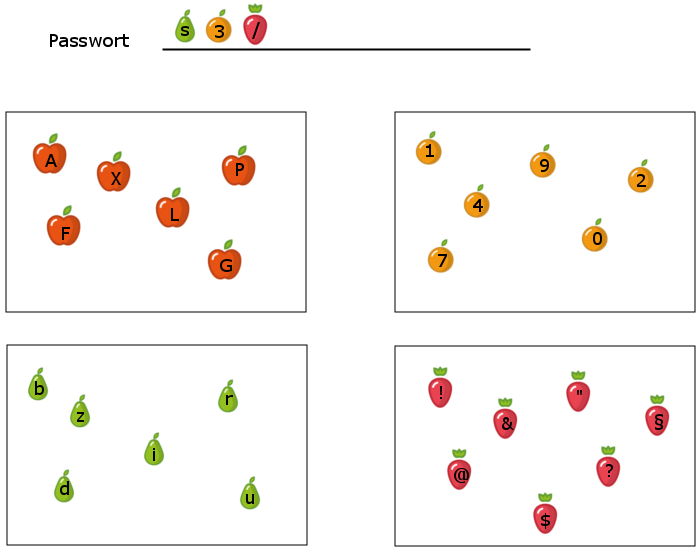
\includegraphics[width=\textwidth]{figures/co-design/fruitsalad-1}
		\caption{\label{fig:co-design:fruitsalad} Fruitsalad: Each character class is represented by a fruit and the user sees a lack of diversity, e.g. if their password only contains lowercase letters.}
	\end{subfigure}
	\begin{subfigure}[!t]{0.49\textwidth}
		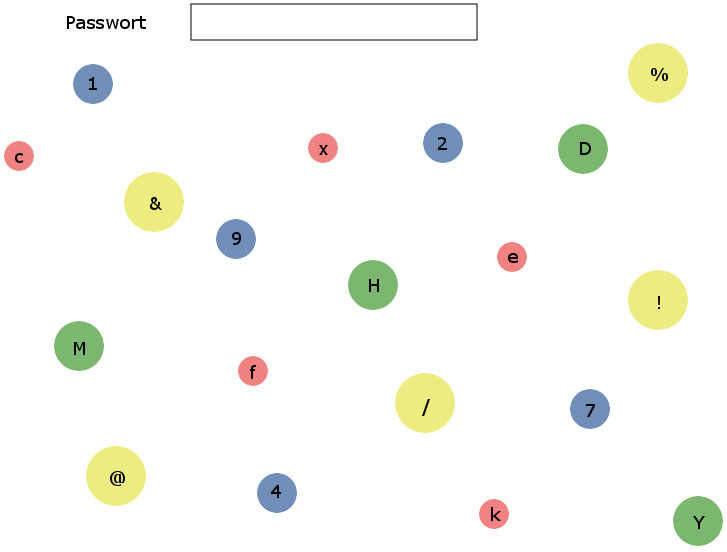
\includegraphics[width=\textwidth]{figures/co-design/bubbles-1}
		\caption{\label{fig:co-design:bubbles-concept}Bubbles: Floating bubbles on the screen that the user pops as they type the password. Symbols are placed in bigger bubbles to be more salient.}
	\end{subfigure}
	\caption{\label{fig:co-design:concepts}Two out of the six concepts that made it to the final feedback iteration.} 
\end{figure}


%- Designs:
%- rewards: beautify page / positive reinforcement from friends (weird suggestions but okay)
%- analogies and requirements feedback: time to crack --> goal: better risk assessment for non-experts. / represent strength contribution of different elements in some way (fruit salad) / vault 
%- playfulness: bubbles / vault / slotmachine to make random character replacements more exciting / 
\subsubsection{``Bubbles'' Prototype}
Participants provided feedback on the six concepts and generally considered the ``bubbles'' concept the best solution to motivate themselves to add more symbols or digits and also make the password longer to watch more bubbles burst. Therefore, we implemented it as an HTML5-based prototype. To add a more game-like feel, we put a score on each character class, and show the currently achieved total score in the GUI. The bubbles move on the screen slowly enough to trace them and their bursts. 

Five of the participants provided a final round of feedback. On the positive side, they felt it intriguing to burst the bubbles. They understood the purpose of the bubbles and the different sizes and colors right away or after typing the first character. Two participants mentioned that it fosters creativity. All said that a system like this would catch their eye and might impact their selection behavior. They also mentioned a number of improvements. For instance, two participants fount the page chaotic and wanted it simplified. The scoring was not transparent either, and three said the bursting animation should be more obtrusive. 

\begin{figure}
	\centering
	\begin{subfigure}[!t]{0.49\textwidth}
		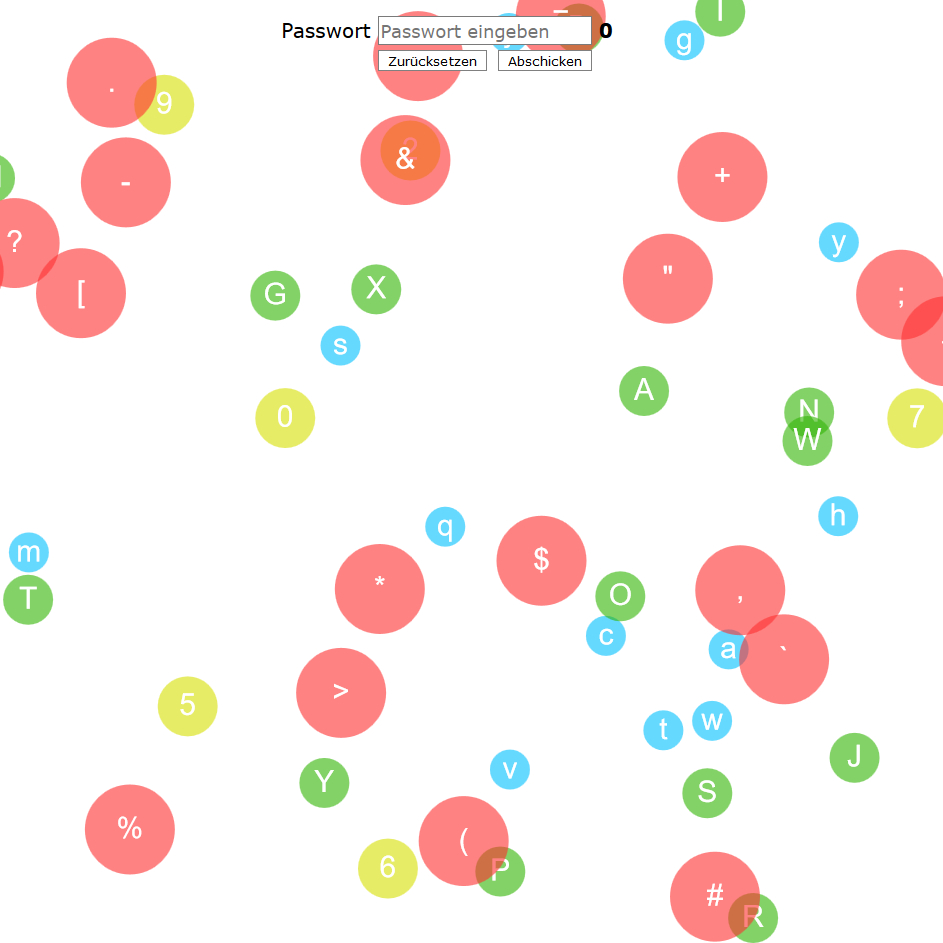
\includegraphics[width=\textwidth]{figures/co-design/bubbles-proto-1}
		\caption{\label{fig:co-design:bubbles-proto-1}}
	\end{subfigure}
	\begin{subfigure}[!t]{0.49\textwidth}
		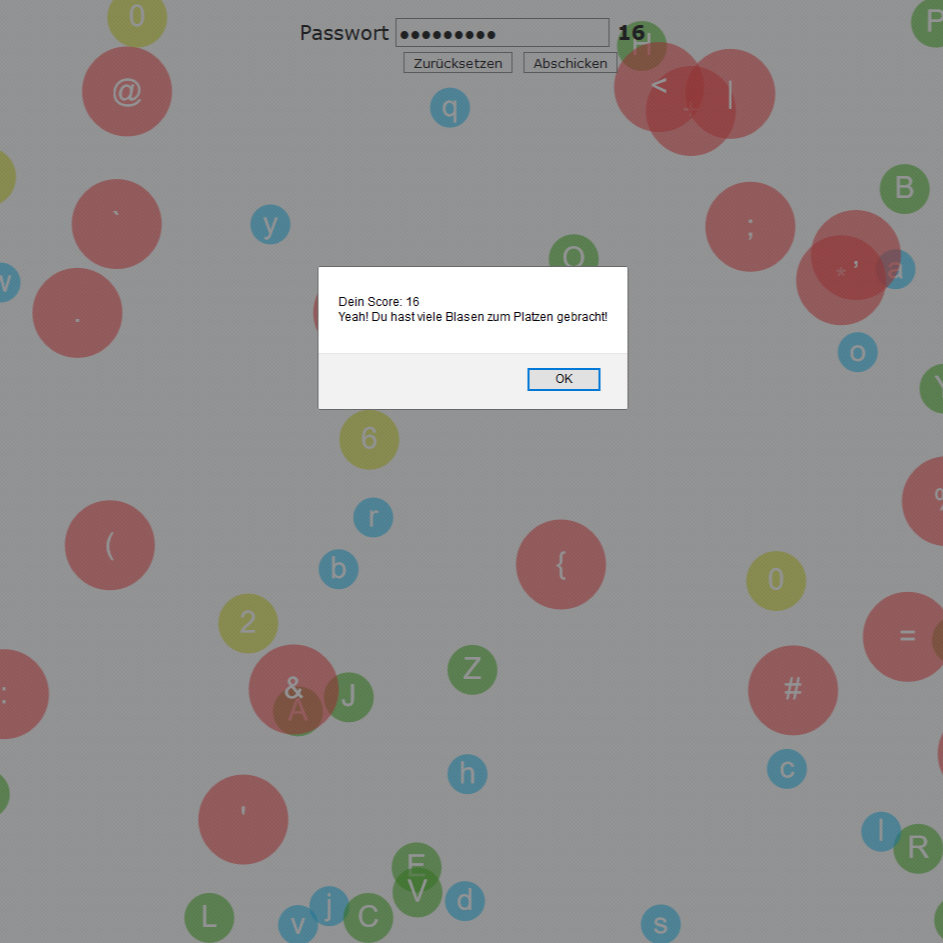
\includegraphics[width=\textwidth]{figures/co-design/bubbles-proto-2}
		\caption{\label{fig:co-design:bubbles-proto-2}}
	\end{subfigure}
	\caption{\label{fig:co-design:bubbles-proto} We made the ``bubbles'' concept into an interactive prototype and gathered a final round of feedback on the outcome and the process.} 
\end{figure}

\subsection{Process Reflection}
What did people say about being involved? What are the opportunities and drawbacks that they saw?
was there something like shared ownership?
- people said it was fun to participate!
- they said it is nice that the final prototype shows elements of their idea generation phase. 
- three said, they would have loved to be involved even more.
- they particularly liked to think about designing for a problem and topic that they had never given too much thought. 
- one participant said they disliked that many ideas were too far fetched and unrealistic. 

\subsection{Learnings about Persuasive Password Interventions}
Discussions among participants and their continuous feedback throughout the design process helped us identify more user needs. We heard that the group had not given the topic much thought before joining the brainstorming session. Many of their ideas went beyond typical password meters, which we highly encouraged. In particular, the concepts show a tendency to visual elements (beautify, pictures, bubbles, fruits) to catch the user's attention. This corresponds to the \textit{show} theme of the requirement-elicitation. The \textit{help} theme was visible especially in the compliance-centered concepts: The ``fruit-salad'' helps people easily identify a potential lack of character diversity. 
While the ``songs'' analogy is a kind of \textit{explanation} of password strength because it gives background information, the ideas did not contain many attempts to explain any more details. Perhaps, participants equated strength with complexity, which their ideas made salient. Finally, the ``bubbles'' concept aimed to boost creativity and thus showed elements of the \textit{help} and \textit{empower} themes. 

%- interesting aspects:
%- a lot of the concepts are visualizable with little text. (emphasize: ``show'' and ``help'')
%- missing: background information. (thus ``explain'' was not visible anymore)
%- empower: not really visible
%kicked out content / structure
% 2
%Ball-bearning exercise
%- add picture of concept: two circles, people on the inner circle interview those on the outer circle who move along after 2 minutes. inner circle gets 1-2 minutes to summarize their findings. 
%- purpose: 
%- first round: own behavior and practices
%- what do (other) people know about password strength and feedback, 
%- what do they do to create passwords
%- share experiences
%- take away: mangling words
%- second round: if they were asked by other people (grandmother, relatives, friends/peers)
%- take away: use context or a good memory as a starting point for your password, e.g. the location and year of a treasured vacation
%- explore potential problems of users, share stories
%- facilitator comments on findings.

%\% 3 
%Idea generation
%- task: ``how would a registration form on a webpage have to look, to help you create a secure password?'' context: email provider
%- quantity!
%- 2x5 minutes in different groups
%- put central topics on whiteboard (17 ideas from both rounds)
%
%\% 4 converge
%- everyone votes for their favorite (2 votes) --> here 3 ideas with 4 votes each were the winners
%- groups of 2 or 3 to build a paper prototype (after a brief explanation what that is)
%
%\% 5 present
%- brief presentation of prototype
%- voting for favorites to inform what we should explore further. 

%(lessons learned and take-aways: 2-3 pages)	
\section{Discussion}
The insights from two rapid methods allow us to derive requirements for persuasive password support, which we put into the context of existing frameworks. 

\subsection{Requirements}
Although the first study was focused on explicit and observable needs, qualitative analysis even brought about more profound needs. Similarly, the second study also helped us understand explicit user needs. Therefore, it was hard to classify the needs, because they were very nuanced. Nonetheless, we show the central characteristics of the requirements in Table \ref{tab:co-design:requirements}.

%%%%%%%%%%%%%%%%%%%%%%%
% REQUIREMENTS TABLE
%%%%%%%%%%%%%%%%%%%%%%%
\begin{table}[htbp]
\begin{tabular}{rp{10cm}ll}
	\# & Requirement & Type & Study \\\hline
	\multicolumn{4}{l}{\textbf{The persuasive tactic needs to ...}} \\\hline
	(1) & Visually indicate current password issues & Explicit & S1 \& S2 \\
	(2) & Offer specific help to diversify passwords & Explicit & S1 \& S2  \\		
	(3) & Be personal & Explicit & S1  \\
	(4) & Provide background information, especially if feedback discounts mental model 
	& Explicit/Observable & S1 \\
	(5) & Stay trustworthy & Observable & S1 \& S2  \\
	(6) & Empower users to act differently & Tacit & S1 \& S2  \\
	(7) & Be straight-forward, easy, and streamlined & Tacit & S1  \\
	(8) & Catch attention, be engaging, foster curiosity & Latent & S2  \\	
	(9) & Open eyes and broaden horizons, e.g. through making unknown coping strategies salient & Latent & S2  \\
	(10) & Avoid habituation effects through surprise and delight & Latent & S2  \\\hline
\end{tabular}
\caption{\label{tab:co-design:requirements} High-level requirements to satisfy different levels of user needs in persuasive password feedback. }
\end{table} %tab:co-design:requirements
% might also do it in this form:
% in the form of user stories
%The user needs to...
% ... sort of a mantra.

\paragraph{Opportunities} Password meters and real-time feedback are the de facto paragon of persuasion in the wild.  Most commonly, they fulfill requirements (1), (2), (4), and (5). For instance, Google's password meter visually encodes password strength with color and bar-size, suggests not using a pet's name, offers extensive background information with a clear call-to-action, and does not jeopardize trustworthiness with extravagant design. On the other hand, it does not necessarily empower users to break habits, is not personalized (what if the user does not have a pet?), and does not account for other ``obvious'' strategies. Academia has produced alternative designs that fulfill requirements (7), (8), and (9), although unusual concepts (like in \cite{Ur2012HowDoesYourPasswordMeasureUp}) were rarely adopted in practice. Empowerment, personalization, and breaking habituation effects have been underexplored, and thus might be worthwhile opportunities for future studies.

\begin{figure}
	\centering
	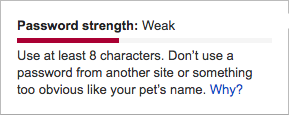
\includegraphics[width=0.4\linewidth]{figures/co-design/google-pw-meter}
	\caption{\label{fig:co-design:google-pw-meter} Google's Password Selection Support UI (March 2018)}
\end{figure}

\subsection{Relation to Current Frameworks}
Most of the themes and requirements show strong links to various persuasion frameworks. In the first study, the qualitative analysis resulted in four essential themes: show, explain, help, empower. Interestingly, there are parallels to \textbf{teaching}. Teachers \textit{show} something new, and then \textit{explain} it in more detail. They \textit{help} students understand it. Often students can then exercise and explore ways to apply their knowledge, i.e. the process \textit{empowers} students to achieve something they could not do before. Forget \etal, who contributed one of the early works on persuasion in cybersecurity, promoted their \acrlong{PAF} as a tool to \textbf{educate} users. All the elements of our qualitative analysis are thus visible in their framework. The requirements in Table \ref{tab:co-design:requirements} represent the themes on a more fine-grained level. Only requirements (8) and (10) are hard to put into the PAF, hence they extend the framework.  
Requirement (8) states that a password support tool should be noticeable and foster curiosity. Generating curiosity can be done in numerous ways, but in this context it relates to Cialdini's \textit{scarcity} principle. The number of ``good'' passwords is much smaller than the number of ``bad'' ones, thus they are a scarce resource. The requirement states that users should realize this and become motivated to access the limited resource. %At the same, time it needs to be easy enough (requirement (7)) and users need to be capable to achieve the goal, which reflects 
%TODO streamline, try to find sub-headings to identify weak structure.

\section{Conclusion}
% goal: understand and externalize the requirements / design space of persuasive interventions
Our goal was to understand the requirements of persuasive password support, especially user needs and expectations. 
% triangulation of methods was feasible and let us derive such requirements
We triangulated methods to rapidly derive feasible requirement that guide future designs of interventions. 
% while survey exhibited explicit idealistic needs, the participatory approach was much more suitable to identify latent needs.
The survey yielded explicit and idealistic needs, like having one's own mental model confirmed by the feedback system. On the other hand, the participatory approach of the second study helped us identify latent needs that would not be detectable in a survey. The results, however, fit together well and solidify the overarching themes ``show'', ``explain'', ``help'', ``empower''. 
% requirements indicate that only verbal or only visual nudging methods are insufficient, they need to be combined
% ur etal recently confirmed this.
Here, we found that participants' expectations of password feedback were nuanced and can thus only be met by combining both verbal and visual support. Feedback was not the only component, because participants showed a need for more guidance in the form of feed\textit{forward}.
% most of the requirements and needs were more or less predictable and already visible in other frameworks, but this specific list helps shaping future desing ideas
The requirements might have been partially predictable even without conducting user research, but tacit and latent needs are uncommonly discussed in related research. Especially the thinking processes and participants' design approaches in the participatory sessions revealed much of what they envisioned in a successful intervention.
% large opportunitites in personalization, empowerment, and breaking habituation. 
Applying the requirements to gauge existing solutions, we identified opportunities for future work in personalization, empowerment, and preventing habituation effects from the same kind of intervention. These are addressed in the following chapters. 

%\vspace*{1cm}\noindent
\fbox{
	\hspace{1cm}
	\parbox[c][12cm]{0.7\linewidth}{
		\section*{Take Aways}
		\begin{itemize}[leftmargin=*]
			\item Triangulation of study methods helped us identify different levels of user needs. Especially the tacit and latent needs are harder to elicit, but participatory design methods were feasible to enhance survey data.
			\item As an explicit need, participants wanted to have their mental models confirmed with password feedback. They become skeptical if the feedback shows unexpected strength results.
			\item Password support systems should meet four essential user needs: \textbf{Show} the current behavior and its consequences visually, \textbf{explain} things that contradict usual mental models, \textbf{help} resolve such dissonances and \textbf{empower} users to act differently.
			%Sounds trivial, but it's important we confirmed it%
		\end{itemize}
	}
	\hspace{1cm}
}


%Kicked out: (Third Step: Hard to justify co-creation):
%\section{Case Study: Jumping on the Bandwagon}
%focus: design rationale and short qualitative evaluation. 
%aim: gauge general feasibility, quantify effects on small scale. 
%\todo{MA von Saron Mebratu}
%Mention that LastPass already has something like this now. -- find out when they introduced it (write them an email) 
%--> nudging via bias seems interesting, but bandwagon is countered with reactance.

%The overarching themes in Study 1 are interestingly just what makes a \textbf{good teacher}: show how it's done and the consequences of actions, explain background info in more depth (which is filtered out anyhow), help students achieve what the teacher showed, and empower them by giving new possibilities to apply knowledge. So this superbly reflects Weirich and Sasse's AND Forget \etal's notion that persuasion is a tool to \textit{educate and teach}. 
%Even in study 2, the final concept is based on a constructivistic teaching paradigm: self-guided exploration and curiosity.

%PAF (teach/learn)
%SDT (motivation)
%Six Weapons (nudging)

%\subsection{Learnings}
%
%- how did this approach help us now?
%- what did we learn?
%- why should we look elsewhere?
%- put solutions / needs into SEHE grid.

%all in all, participants in the survey were somewhat too optimistic compared to quantitative / empirical results.

%the requirements should somehow be related to what's to come in the decoy chapter. E.g. the suggestive and trustworthiness of suggestions / feedback was challenged by first participants.

%The way people designed interventions shows their mental models and lets us inform our own design decisions. We are not the users and simply ``knowing it better'' won't get us very far. We have to pick people up where they are to have a chance in designing effective nudges. 

%--> empowerment... TODO.
%hard to explain problem space / pw strength to users so briefly. tension. when and for whom. 


% why isn't this trivial?
% where is the nudging part? 
